%% nicht vergessen draft raus zu nehmen, um echte Bilder einzubinden und die Problem-Vierecke verschwinden zu lassen
\documentclass[11pt,a4paper,oneside,svgnames]{report}

\usepackage[british]{babel}
\usepackage[utf8]{inputenc}
\usepackage[T1]{fontenc}
\usepackage{ae}
\usepackage[table]{xcolor}
\usepackage{colortbl}
\usepackage{graphicx}
\usepackage{tikz}
\usepackage{kpfonts}
\usepackage[explicit]{titlesec}
\usepackage[acronym,toc,nonumberlist,style=tree]{glossaries}
\usepackage{amssymb}

\definecolor{tableHead}{HTML}{FF00FF}
\definecolor{tableEven}{HTML}{FF0000}
\definecolor{tableOdd}{HTML}{00FF00}

\makeglossaries

\newglossaryentry{pin}{name=PIN,description={Personal Identification Number},plural=PINs, first={Personal Identification Number (PIN)}}

\newacronym{led}{LED}{light-emitting diode}


\begin{document}

\title{Software Requirements Specifications\\ for\\ Project ``BookExpress''}
\author{Marc A. Harnos\\ {mharnos@gmail.com} \and Joscha Rapp\\ {jraxxo@gmail.com} \and Christian Schulz\\ {crs.s@gmx.net}}
\date{October 2012}
\maketitle
\tableofcontents

\chapter*{Document History}
\begin{tabular}{|l|l|l|l|}
\hline 
Editor(s) & Date & Purpose of Editing & Version \\ 
\hline 
Harnos, Rapp, Schulz & 2012-10-01 & Initial Document Creation & v0.01 \\ 
\hline 
\end{tabular} 

\chapter{Product Purpose}
To handle the addition of new books and the distribution in a better way, "BookExpress" asked us to develop an IT solution to optimize the idle time and labour usage by getting rid of the current, deprecated system. Furthermore one important goal of the software solution is to be very user friendly and easy to use; also there should be remote access implemented, so several customers can access the software at once and distribution partners can access and keep their book stock up to date.
\section{Obligatory Requirements (``must have'')}
\subsection{Communication with Publishers}
The direct connection between the \textbf{publishers} and BookExpress shall be implemented by providing a web interface for the publishers.\\
\begin{itemize}
\item As each publisher also has a PIN, it will be used as the account name for the interface.
\item The web interface has to provide the following features for the publisher: maintain the book database (add books, remove books, edit book data), edit their personal data, view statistics on how often which books are bought
\item The interface has to be comfortably accessible from mobile devices as well, the data that is transmitted should be minimal\\
\end{itemize}
\subsection{Communication with Customers}
The direct connection between the \textbf{customers} and BookExpress shall also be implemented by providing a web interface for the customers.\\
\begin{itemize}
\item As each customer already has a unique identifier, the PIN, we will use it as an account name for the login.
\item The web interface has to provide the following features: view catalogue and stock, submit orders, view  the current state of their orders and cancel them (if they haven't been shipped yet)
\item The system has to assign a unique ID to each order, ideally incorporating the PIN of the customer
\item The interface has to be comfortably accessible from mobile devices as well, the data that is transmitted should be minimal\\
\end{itemize}
\subsection{Internal Administration}
The employees of BookExpress shall be provided a web interface as well. 
\begin{itemize}
\item Each employee will get a unique user ID to log into the web interface. Ideally, this will be formatted along the lines of surname.name or something similar.
\item The web interface must provide the following features for the employees: processing, editing and cancellation  of submitted orders, directly contact the customers and publishers as well as the truck fleet and the warehouse
\item Furthermore, the underlying system shall generate logfiles with login times, error codes and statistics (e.g. which books are ordered the most and by whom) for the publishers and the accounting and IT department / tech support.
\item The interface has to be comfortably accessible from mobile devices as well, the data that is transmitted should be minimal\\ 
\end{itemize}
\subsection{Support}
\begin{itemize}
\item The system should be as automatic as possible - we need a good, user-oriented manual.
\item Additionally, a context-sensitive help tool has to be implemented in the interface itself. 
\item Moreover, As we want to make sure that the system is as reliable as possible, we will need a dedicated support team that is available 24/7 and can be dispatched in less than 2 hours to fix critical issues.
\end{itemize}

\section{Optional Requirements (``nice to have'')}
\begin{itemize}
\item Book Stores should be able to save recurring orders
\item Book Stores should be notified when the delivery of their order is imminent\\
\end{itemize}

\section{Non-Requirements (``need not have'')}
\begin{itemize}
\item The software should not allow final customers to buy books. It is only intended for retailers.
\item Moreover, invoices are generated elsewhere, as well as financial reports, so the system should not interfere with that.\\
\end{itemize}
\chapter{Product Environment}
The Product takes the orders from the book stores and files them into the system, so that they can be prepared for shipping. For different sized book stores there should be several account types with separate functionality and different options for packaging and ordering. The targeting groups of the software solution are the book store owners(our consumers), the assistants of "BookExpress" and the distribution partners.
\section{Application Area}
The new IT system should replace the old system and provide administrative and commercial functions to relieve the employees of unnecessarily complex administrative tasks. Certain processes can be handled without any interaction at all, e.g. if a book runs low in stock, the system will automatically order new copies from the publisher.
\section{User Groups}
\begin{itemize}
\item BookExpress commercial employees
\item BookExpress IT employees
\item Publishers
\item Book Stores
\end{itemize}
\section{Operating Conditions}

\chapter{Product Overview}
The products environmental diagram.

\begin{figure}[h!]
 \begin{center}
  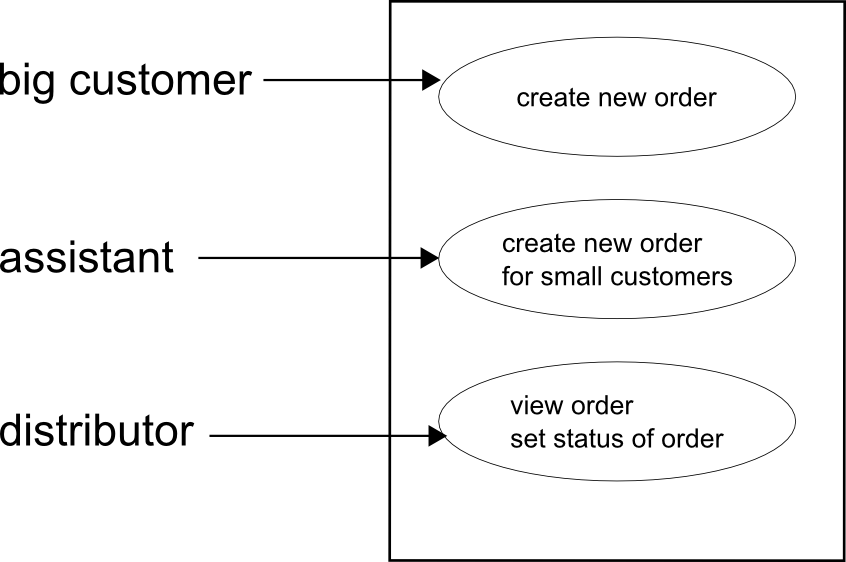
\includegraphics[scale=0.8]{images/umweltdiagramm.png}
 \end{center}
 \caption{The environmental view of the product}
\end{figure}


\chapter{Product Functions}

\section{Internal}
\subsection{Employees of ``BookExpress''}

\noindent
\begin{tabular}{p{1.5cm}p{3cm}p{8cm}}
/PF10/	& \textbf{Process}	& Register Publisher or Book Shop (client)\\
		& \textbf{Actor(s)} & BookExpress employee\\
		& \textbf{Category} & Must have\\
		& \textbf{Description}	 & A Book Express employee creates an account for a book shop or publisher after both business partners have signed a contract handling the business relations.\\
		& \textbf{Goal} & The contract partner should have an account to log into the Software. After registration through the Book Express employee, the contract partner will be send a verification and its 
		 information via email.\\
		& \textbf{Preconditions} & Contract signed\\
		& \textbf{Postcondition success} & Successfully created account\\
		& \textbf{Postcondition failure} & Unsuccessful in creating an account\\
		& \textbf{Trigger} & Menu option "register new client" (Software)\\
		& \textbf{Sequence} & Input relevant data and contractor details into the managements system\\
		& & Save the signed contract on the server\\
		& & Register a new client by creating a new PIN in the database\\
		& & Send verification and account information to the contractor\\
\hfill \\
\end{tabular}

\noindent
\begin{tabular}{p{1.5cm}p{3cm}p{8cm}}
/PF20/	& \textbf{Process} & Update account information\\
		& \textbf{Actor(s)} & BookExpress employee\\
		& \textbf{Category} & \\
		& \textbf{Description}	 & The clients data is outdated and needs to be updated\\
		& \textbf{Goal} & Client data is updated\\
		& \textbf{Preconditions} & Client exists in database\\
		& \textbf{Postcondition success} & Client data is updated and a notification mail is sent to the client.\\
		& \textbf{Postcondition failure} & Client data is not updated but rolled back to the previous state. Notification with problem report is shown to the employee.\\
		& \textbf{Trigger} & Menu option "Update account" (Software)\\
		& \textbf{Sequence} & Edit specific data\\
		& & Submit edited data to the server\\
\hfill \\
\end{tabular}

\noindent
\begin{tabular}{p{1.5cm}p{3cm}p{8cm}}
/PF02/	& \textbf{Process} & Delete account\\ 
		& \textbf{Actor(s)} & BookExpress Employee\\ 
		& \textbf{Category} & \\
		& \textbf{Description}	 & Client gets deleted due to resignation of the contract\\ 
		& \textbf{Goal} & Delete client from the system\\
		& \textbf{Preconditions} & Client exists in database\\
		& & Contract is being resigned by one of the contractors\\
		& \textbf{Postcondition success} & Client is deleted from the system\\
		& \textbf{Postcondition failure} & Client could not be deleted because of existing orders\\
		& \textbf{Trigger} & Menu option "delete client" (Software)\\
		& \textbf{Sequence} & Choose client\\
		& & Check if client is deletable (i.e. no existing orders)\\
		& & Send notification mail to client\\
		& & Delete client\\
\hfill \\		
\end{tabular}

\noindent
\begin{tabular}{p{1.5cm}p{3cm}p{8cm}}
	 /PF/	& \textbf{Process} & Client places order\\ 
		& \textbf{Category} & \\
		& \textbf{Actor(s)} & BookExpress employee, client\\ 
		& \textbf{Description}	 & A client orders book via telephone\\ 
		& \textbf{Goal} & Order is placed in an order queue\\
		& \textbf{Preconditions} & Client exists in database\\
		& & Client is authorized\\
		& \textbf{Postcondition success} & Order is placed in an order queue\\
		& \textbf{Postcondition failure} & -\\
		& \textbf{Trigger} & Client initiates order process by calling an BookExpress employee\\
		& & BookExpress employee triggers manual order process\\
		& \textbf{Sequence} & BookExpress employee selects client in Software\\
		& & BookExpress employee enters ordered book into the system\\
		& & Order is placed in order queue\\
		& & Order notification containing detailed report is sent to client\\
\hfill \\
\end{tabular}

\noindent
\begin{tabular}{p{1.5cm}p{3cm}p{8cm}}
	 /PF/	& \textbf{Process} & Validate order\\ 
		& \textbf{Category} & \\
		& \textbf{Actor(s)} & System\\ 
		& \textbf{Description}	 & Order is checked for validation\\ 
		& \textbf{Goal} & The software checks every order for validation and confirms it to the client. BookExpress knows about every orders validation status.\\
		& \textbf{Preconditions} & Order is in order queue\\
		& \textbf{Postcondition success} & Client receives a confirmation email\\
		& \textbf{Postcondition failure} & Client receives a problem report about invalid order\\
		& \textbf{Trigger} & Order was placed and exists in order queue\\
		& \textbf{Sequence} & System  gathers details and checks whether order is valid or not\\
		& & System sends mail to client\\
\hfill \\
\end{tabular}

\noindent
\begin{tabular}{p{1.5cm}p{3cm}p{8cm}}
	 /PF/	& \textbf{Process} & Stock Update\\ 
		& \textbf{Category} & Must have\\
		& \textbf{Actor(s)} & System/BookExpress employee\\ 
		& \textbf{Description}	 & The employee in charge of the stock checks the availability of all books and updates the stock accordingly.\\ 
		& \textbf{Goal} & Check succeeds\\
		& \textbf{Preconditions} & Order is placed or BookExpress employee initiates check\\
		& \textbf{Postcondition success} & Books which are nearly out of stock get displayed as a list\\
		& \textbf{Postcondition failure} & -\\
		& \textbf{Trigger} & Stock check is initiated\\
		& \textbf{Sequence} & Check if a book is available in an sufficient amount\\
		& & Make a list of all books which need to be ordered\\
		& & Submit list to system\\
\hfill \\
\end{tabular}

\noindent
\begin{tabular}{p{1.5cm}p{3cm}p{8cm}}
	 /PF/	& \textbf{Process} & Forward order to Logistics\\ 
		& \textbf{Category} & \\
		& \textbf{Actor(s)} & System\\ 
		& \textbf{Description}	 & A validated order gets forwarded to Logistics\\ 
		& \textbf{Goal} & Logistics proceeds processing the order\\
		& \textbf{Preconditions} & Order is valid\\
		& \textbf{Postcondition success} & Logistics processes delivery\\
		& \textbf{Postcondition failure} & Order could not be forwarded to Logistics\\
		& \textbf{Trigger} & Order is validated\\
		& \textbf{Sequence} & Send order information/details to Logistics\\
\hfill \\
\end{tabular}

\noindent
\begin{tabular}{p{1.5cm}p{3cm}p{8cm}}
/PF/	& \textbf{Process} & Deliver order\\
		& \textbf{Actor(s)} & System\\
		& \textbf{Category} & \\
		& \textbf{Description}	 &  The order is send to the book store\\
		& \textbf{Goal} & Deliver ordered books\\
		& \textbf{Preconditions} & Order is valid\\
		& & Books are available in stock\\
		& \textbf{Postcondition success} & Order is marked as sent\\
		& \textbf{Postcondition failure} & Order could not be marked as sent\\
		& \textbf{Trigger} & Forward order to Logistics\\
		& \textbf{Sequence} & Check if books are in stock\\
		& & Receive book store information\\
		& & Sent order to book store\\
		& & Mark order as sent\\
		
\hfill \\
\end{tabular}

\noindent
\begin{tabular}{p{1.5cm}p{3cm}p{8cm}}
/PF/	& \textbf{Process} & Confirm delivery\\
		& \textbf{Actor(s)} & Employee (Logistics)\\
		& \textbf{Category} & \\
		& \textbf{Description}	 & Logistics confirms the correct delivery of an order\\
		& \textbf{Goal} & Delivery is successful\\
		& \textbf{Preconditions} & Order is marked as sent\\
		& \textbf{Postcondition success} & Order is marked as delivered\\
		& \textbf{Postcondition failure} & Order could not be marked as delivered\\
		& \textbf{Trigger} & Deliver order\\
		& \textbf{Sequence} & Get delivery status\\
		& & Mark order as delivered if delivery status is "successfully delivered"
		
\hfill \\
\end{tabular}

\noindent
\begin{tabular}{p{1.5cm}p{3cm}p{8cm}}
/PF/	& \textbf{Process} & BookExpress Order\\
		& \textbf{Actor(s)} & BookExpress employee\\
		& \textbf{Category} & \\
		& \textbf{Description}	 & The Employee orders a number of books from the publisher\\
		& \textbf{Goal} & Order books from a publisher\\
		& \textbf{Preconditions} & need for new books\\
		& \textbf{Postcondition success} & Books are ordered and publisher gets an notification mail\\
		& \textbf{Postcondition failure} & -\\
		& \textbf{Trigger} & BookExpress employee initates an order\\
		& \textbf{Sequence} & Select books from list or search TODO /PF/\\
		& & Submit list to publisher\\
		
\hfill \\
\end{tabular}

\noindent
\begin{tabular}{p{1.5cm}p{3cm}p{8cm}}
/PF/	& \textbf{Process} & Create an invoice\\
		& \textbf{Actor(s)} & System\\
		& \textbf{Category} & \\
		& \textbf{Description}	 & The system creates an invoice after TODO /PF/ order is valid\\
		& \textbf{Goal} & Documenting order and deliver it with invoice\\
		& \textbf{Preconditions} & Order is valid\\
		& \textbf{Postcondition success} & Invoice successfully created\\
		& \textbf{Postcondition failure} & Invoice could not be created\\
		& & Check information about order\\
		& \textbf{Trigger} & Order is valid TODO /PF/\\
		& \textbf{Sequence} & Create an entry in database\\
		& & List the ordered books with price\\
		& & List tax to invoice\\
		
\hfill \\
\end{tabular}

\noindent
\begin{tabular}{p{1.5cm}p{3cm}p{8cm}}
/PF/	& \textbf{Process} & Send invoice\\
		& \textbf{Actor(s)} & System\\
		& \textbf{Category} & \\
		& \textbf{Description}	 & The invoice is send to the book store via mail\\
		& \textbf{Goal} & Inform the book shop\\
		& \textbf{Preconditions} & Successful created invoice\\
		& \textbf{Postcondition success} & Book store receives a notification mail\\
		& \textbf{Postcondition failure} & -\\
		& \textbf{Trigger} & Creation of an invoice\\
		& \textbf{Sequence} & Get invoice\\
		& & Send invoice to book store
		
\hfill \\
\end{tabular}

\noindent
\begin{tabular}{p{1.5cm}p{3cm}p{8cm}}
/PF/	& \textbf{Process} & Backup\\
		& \textbf{Actor(s)} & System\\
		& \textbf{Category} & \\
		& \textbf{Description}	 & A backup of the complete databases must be done. This should happen periodically and save all data on a server.\\
		& \textbf{Goal} & In case of a crash, every data must be saves as a preventative backup\\
		& \textbf{Preconditions} & Server for the backup\\
		& \textbf{Postcondition success} & Successful backup in periodical intervals\\
		& \textbf{Postcondition failure} & A notification will be send to the administrator of the system\\
		& \textbf{Trigger} & Configured time to start a backup\\
		& \textbf{Sequence} & Start Backup\\
		& & Place backup on the backup server
		
\hfill \\
\end{tabular}

\section{External}
\subsection{Book Stores (``Clients'')}

\subsection{Book Stores and Publishers}

\noindent
\begin{tabular}{p{1.5cm}p{3cm}p{8cm}}
/PF/	& \textbf{Process} & Login\\
		& \textbf{Actor(s)} & Book store/publisher\\
		& \textbf{Category} & Must have\\
		& \textbf{Description}	 & The user logs on with his PIN and password\\
		& \textbf{Goal} & Provide a fully functional system to the user\\
		& \textbf{Preconditions} & Existing account\\
		& \textbf{Postcondition success} & Successful login\\
		& \textbf{Postcondition failure} & Unsuccessful login caused by a wrong PIN or password\\
		& \textbf{Trigger} & Menu Option "Login"\\
		& \textbf{Sequence} & Enter PIN\\
		& & Enter password\\
		& & Validity of data is checked by the System\\
		& & Login successful or display an error message in case of unsuccessful login
		
\hfill \\
\end{tabular}

\noindent
\begin{tabular}{p{1.5cm}p{3cm}p{8cm}}
/PF/	& \textbf{Process} & Update account information\\
		& \textbf{Actor(s)} & Book store/publisher\\
		& \textbf{Category} & Must have\\
		& \textbf{Description}	 & The user is able to edit/update its account information (e.g. address, correspondent etc.)\\
		& \textbf{Goal} & User is able to update changes\\
		& \textbf{Preconditions} & User is logged on\\
		& \textbf{Postcondition success} & Updating the account succeeded\\
		& \textbf{Postcondition failure} & Updating the account failed\\
		& \textbf{Trigger} & Menu option "Update account"\\
		& \textbf{Sequence} Edit specific data\\
		& & System checks correctness of data (e.g. email format etc.)\\
		& & Submit edited data to the server\\
		
\hfill \\
\end{tabular}

\noindent
\begin{tabular}{p{1.5cm}p{3cm}p{8cm}}
/PF/	& \textbf{Process} & Logout\\
		& \textbf{Actor(s)} & Book store/publisher\\
		& \textbf{Category} & Must have\\
		& \textbf{Description}	 & User logs out\\
		& \textbf{Goal} & User is logged out\\
		& \textbf{Preconditions} & User is logged in\\
		& \textbf{Postcondition success} & Successful logout\\
		& \textbf{Postcondition failure} & Unsuccessful logout caused by an abort of the user\\
		& \textbf{Trigger} & Menu option "Logout"\\
		& \textbf{Sequence} & User confirms to log out\\
		& & The system terminates the current session\\
\hfill \\
\end{tabular}


\subsection{Book Stores (``Clients'')}

\noindent
\begin{tabular}{p{1.5cm}p{3cm}p{8cm}}
	 /PF/	& \textbf{Process} & Search for a book/show catalogue\\ 
		& \textbf{Category} & Must have\\
		& \textbf{Actor(s)} & Client\\ 
		& \textbf{Description}	 & Client searches for a book to add it to his order\\ 
		& \textbf{Goal} & Searching for a book succeeded\\
		& \textbf{Preconditions} & Client is logged into the system\\
		& \textbf{Postcondition success} & Book is being found\\
		& & Display items and options\\
		& \textbf{Postcondition failure} & Book could not be found\\
		& & Display notification\\
		& \textbf{Trigger} & Menu option "find books" (Software)\\
		& \textbf{Sequence} & Enter ISBN/title/author/genre in search bar\\
		& & Hit the "Search"-Button\\
		& & Choose book from list to add it to the order\\
\hfill \\
\end{tabular}

\noindent
\begin{tabular}{p{1.5cm}p{3cm}p{8cm}}
/PF/	& \textbf{Process} & Book Store Order\\ 
		& \textbf{Category} & Must have\\
		& \textbf{Actor(s)} & Book Store Employee\\ 
		& \textbf{Description}	 & The Book Store orders a book from BookExpress.
This can either happen through a constant connection where every order is individually processed or the store can choose to collect orders internally and send them
as one big order every day.\\ 
		& \textbf{Goal} & Order is placed\\
		& \textbf{Preconditions} & Client is successfully logged into the web interface\\
		& & Connection to BookExpress server is established\\
		& \textbf{Postcondition success} & Order is delivered to BookExpress  and added to the order queue\\
		& \textbf{Postcondition failure} & Order is saved as draft and client gets a notification\\
		& \textbf{Trigger} & Menu Option "create new order" (Web interface)\\
		& \textbf{Sequence} & Client adds books to order (via book search or ISBN)\\
		& & Client specifies amount for every book\\
		& & Client submits order to server\\
		& & Order is in the order queue\\
\hfill \\
\end{tabular}

\noindent
\begin{tabular}{p{1.5cm}p{3cm}p{8cm}}
/PF/	& \textbf{Process} & Change order\\
		& \textbf{Actor(s)} & Book store\\
		& \textbf{Category} & Must have\\
		& \textbf{Description}	 & As long as the order is not validated, the user can change information\\
		& \textbf{Goal} & User can correct an order\\
		& \textbf{Preconditions} & Order exists and user is logged in\\
		& \textbf{Postcondition success} & Order information successfully changed\\
		& \textbf{Postcondition failure} & Order information could not be changed because the order is already being validated\\
		& \textbf{Trigger} & Menu option "Change order"\\
		& \textbf{Sequence} & Select order to be changed\\
		& & System checks validity status of the order\\
		& & If not validated, user can change order information\\
		& & Submit changes to the System\\
		& & User receives a confirmation mail\\
		
\hfill \\
\end{tabular}

\noindent
\begin{tabular}{p{1.5cm}p{3cm}p{8cm}}
/PF/	& \textbf{Process} & Cancel Order\\
		& \textbf{Actor(s)} & Book Store Employee\\
		& \textbf{Category} & Must have\\
		& \textbf{Description}	 & The employee at the book store can cancel the order if it hasn’t been shipped yet\\
		& \textbf{Goal} & Current orders can be cancelled\\
		& \textbf{Preconditions} & Order exists\\
		& \textbf{Postcondition success} & Order successfully cancelled. Book Store receives a confirmation mail\\
		& \textbf{Postcondition failure} & Book Store receives a problem report\\
		& \textbf{Trigger} & Menu option "cancel order"\\
		& \textbf{Sequence} & Select order to cancel\\
		& & Check whether order isn't shipped yet\\
		& & Cancel order
		
\hfill \\
\end{tabular}

\noindent
\begin{tabular}{p{1.5cm}p{3cm}p{8cm}}
/PF/	& \textbf{Process} & Tracking System\\
		& \textbf{Actor(s)} & Book Store Employee\\
		& \textbf{Category} & Must have\\
		& \textbf{Description}	 & The employee at the book store can look up at which stage his order is right now, e.g. processing or shipping to BookExpress/the book store.\\
		& \textbf{Goal} & Look up order information/status\\
		& \textbf{Preconditions} & Order exists\\
		& \textbf{Postcondition success} & Employee receives information/status of order\\
		& \textbf{Postcondition failure} & -\\
		& \textbf{Trigger} & Menu option "tracking system"\\
		& \textbf{Sequence} & Select order to track\\
		
\hfill \\
\end{tabular}

\subsection{Publishers}

\noindent
\begin{tabular}{p{1.5cm}p{3cm}p{8cm}}
/PF10/	& \textbf{Process} & Inventory maintenance\\
		& \textbf{Actor(s)} & Publisher\\
		& \textbf{Category} & Must have\\
		& \textbf{Description}	 & Publishers can update their inventory list
(i.e. the list of available books) either via mail or using the direct connection over the web-based interface.\\
		& \textbf{Goal} & Updated inventory list\\
		& \textbf{Preconditions} & Publisher exists\\
		& \textbf{Postcondition success} & Send success mail to publisher\\
		& \textbf{Postcondition failure} & Send problem report to publisher\\
		& \textbf{Trigger} & Menu option "inventory maintenance" (Software) or via mail\\
		& \textbf{Sequence} & Edit inventory list (i.e with TODO book search)\\
		& & Submit list to server
		
\hfill \\
\end{tabular}

\chapter{Product Data}
\section{User Data}
\subsection{Book Stores}

\rowcolors{1}{tableEven}{tableOdd}
\begin{tabular}{llp{10cm}}
\cellcolor{white}/PD20/	& \textbf{Data}			& Book Store Data\\
\cellcolor{white}		& \textbf{Composition}	& Name, PIN, Address, Correspondent, E-Mail Address, Phone Number, Contract Data\\
\cellcolor{white}		& \textbf{Size}		& approx 10,000\\
\cellcolor{white}		& \textbf{Traffic}		& Low\\
\end{tabular} 
\subsection{Publishers}
\begin{tabular}{llp{10cm}}
\cellcolor{white}/PD30/	& \textbf{Data}			& Publisher Data\\
\cellcolor{white}		& \textbf{Composition}	& Name, PIN, Address, Correspondent, E-Mail Address, Phone Number, Contract Data\\
\cellcolor{white}		& \textbf{Size}		& approx 15,000\\
\cellcolor{white}		& \textbf{Traffic}		& Low\\
\end{tabular} 
\section{Order Data}
\begin{tabular}{llp{10cm}}
\cellcolor{white}/PD40/	& \textbf{Data}			& Order Data\\
\cellcolor{white}		& \textbf{Composition}	& PIN, ISBN, Amount, Price, Date, Current Ordering State\\
\cellcolor{white}		& \textbf{Size}		& 500,000\\
\cellcolor{white}		& \textbf{Traffic}		& Very High\\
\cellcolor{white}\hfill \\
\cellcolor{white}/PD41/	& \textbf{Data}			& Order Data History\\
\cellcolor{white}		& \textbf{Composition}	& PIN, ISBN, Amount, Price, Date\\
\cellcolor{white}		& \textbf{Size}		& 2,500,000\\
\cellcolor{white}		& \textbf{Traffic}		& High\\
\end{tabular} 
\section{Internal Data}
\subsection{Book Stock}
\begin{tabular}{llp{10cm}}
\cellcolor{white}/PD10/	& \textbf{Data}			& Book Data\\
\cellcolor{white}		& \textbf{Composition}	& ISBN, UPC/EAN, Title, Author, Publisher, Availability\\
\cellcolor{white}		& \textbf{Size}		& approx 1,500,000\\
\cellcolor{white}		& \textbf{Traffic}		& Average\\
\end{tabular} 
\subsection{Truck Information}
\begin{tabular}{llp{10cm}}
\cellcolor{white}/PD50/	& \textbf{Data}			& Truck Fleet Data\\
\cellcolor{white}		& \textbf{Composition}	& Driver, Registration Number, Status\\
\cellcolor{white}		& \textbf{Size}		& 1,000\\
\cellcolor{white}		& \textbf{Traffic}		& Average\\
\end{tabular} 

\chapter{Product Performance}
\section{System}
\noindent
\begin{tabular}{llp{10cm}}
\cellcolor{white}/PP10/	& \textbf{Type}			& System (Web Interface)\\
\cellcolor{white}		& \textbf{Description}	& The Web Interface should be always reachable during business hours, but also 24/7 for quick changes. The availability outside business hours can be less than 100\% but should not fall below 99.7\%.\\
\cellcolor{white}		\hfill \\
\end{tabular}

\noindent
\begin{tabular}{llp{10cm}}
\cellcolor{white}/PP30/	& \textbf{Type}			& System (Order Processing)\\
\cellcolor{white}		& \textbf{Description}	& The order processing should always be reachable, confirming (or informing about, in case of error) any order.\\
\cellcolor{white}		\hfill \\
\end{tabular}

\noindent
\begin{tabular}{llp{10cm}}
\cellcolor{white}/PP40/	& \textbf{Type}			& System\\
\cellcolor{white}		& \textbf{Description}	& The System in general should be reliable and responsive all the time, taking not longer than 1-3 seconds for any request.\\
\cellcolor{white}		\hfill \\
\end{tabular}

\noindent
\begin{tabular}{llp{10cm}}
\cellcolor{white}/PP50/	& \textbf{Type}			& System\\
\cellcolor{white}		& \textbf{Description}	& The response time criteria should also be met, when the processing limit of max. 2.000 simultaneous orders is reached.\\
\cellcolor{white}		\hfill \\
\end{tabular}

\section{Database}

\noindent
\begin{tabular}{llp{10cm}}
\cellcolor{white}/PP20/	& \textbf{Type}			& Database (DB Connection)\\
\cellcolor{white}		& \textbf{Description}	& A Connection to the database should never be lost, an average uptime of 99.99\% has to be reached to satisfy any part of the system, currently needing data.\\
\cellcolor{white}		\hfill \\
\end{tabular}

\noindent
\begin{tabular}{llp{10cm}}
\cellcolor{white}/PP21/	& \textbf{Type}			& Database (DB Backup)\\
\cellcolor{white}		& \textbf{Description}	& A database backup has to be initiated meeting the guidelines on general backup, also ensuring a consistent and complete history of any processed orders and any critical data.\\
\cellcolor{white}		\hfill \\
\end{tabular}

\section{Security}
\noindent
\begin{tabular}{llp{10cm}}
\cellcolor{white}/PP60/	& \textbf{Type}			& Security (Stock Availability)\\
\cellcolor{white}		& \textbf{Description}	& Stock items should always be able to be ordered, ensuring fast delivery on order.\\
\cellcolor{white}		\hfill \\
\end{tabular}

\noindent
\begin{tabular}{llp{10cm}}
\cellcolor{white}/PP61/	& \textbf{Type}			& Security (Connection)\\
\cellcolor{white}		& \textbf{Description}	& Any connection issued to the system and between system components should be at least encrypted with 256 bit SSL.\\
\cellcolor{white}		\hfill \\
\end{tabular}

\noindent
\begin{tabular}{llp{10cm}}
\cellcolor{white}/PP62/	& \textbf{Type}			& Security (Database)\\
\cellcolor{white}		& \textbf{Description}	& The database should be on an encrypted device, securing personal customer data.\\
\cellcolor{white}		\hfill \\
\end{tabular}

\chapter{Quality Requirements}

\rowcolors{1}{tableEven}{tableOdd}
\begin{tabular}{|lllll|}
\hline
\cellcolor{tableHead}Product Quality & \cellcolor{tableHead}excellent & \cellcolor{tableHead}good & \cellcolor{tableHead}normal & \cellcolor{tableHead}not applicable \\ 
\hline
Functionality &  &  &  &  \\ 
suitability &  & \checkmark &  &  \\ 
correctness & \checkmark &  &  &  \\ 
interoperability &  & \checkmark &  &  \\ 
conformity &  & \checkmark &  &  \\ 
security & \checkmark &  &  &  \\ 
Reliability &  &  &  &  \\ 
maturity &  & \checkmark &  &  \\ 
error tolerance &  & \checkmark &  &  \\ 
re-invoking & \checkmark &  &  &  \\ 
Usability &  &  &  &  \\ 
comprehensibility &  & \checkmark &  &  \\ 
learnability &  &  & \checkmark &  \\ 
ease of use &  & \checkmark &  &  \\ 
Efficiency &  &  &  &  \\ 
time behaviour & \checkmark &  &  &  \\ 
resource use &  &  & \checkmark &  \\ 
Maintainability &  &  &  &  \\ 
easy to analyse &  & \checkmark &  &  \\ 
easy to modify &  &  & \checkmark &  \\ 
stability & \checkmark &  &  &  \\ 
testability &  &  &  & \checkmark \\ 
Installability &  &  &  &  \\ 
adaptability &  &  & \checkmark &  \\ 
easy to install &  &  & \checkmark &  \\ 
conformity &  & \checkmark &  &  \\ 
exchangeability &  &  &  & \checkmark \\
\hline
\end{tabular}

\chapter{User Interface}
\section{Client Application (for clerks)}
\section{Web Interface (for customers)}

\chapter{Non-Functional Requirements}
\chapter{Technical Product Environment}
\section{Software}
\section{Hardware}
\section{Orgware}
\section{Interfaces (product)}

\chapter{Special Requirements for the Development Environment}
\section{Software}
\section{Hardware}
\section{Orgware}
\section{Interfaces (development)}

\chapter{Subproducts and Subsystems}
\section{Server}
\section{Web Interface / Web Service}
\section{Client Application}

\chapter{Additional Specifications and Stipulations}
\chapter{Appendices}
\printglossaries

\end{document}